% -*- TeX-master: "multi" -*-

\section{Examples}
\label{def:Examples}

This section contains examples employing the \multi\ package for \SbmlLevelThree.

%----------------------------------------------------------------
\subsection{Example: \ExCompartment, \SpeciesType, and \ExSpecies}
\label{def:Example:CompartmentSpeciesTypeSpecies}

\begin{figure}[htb]
  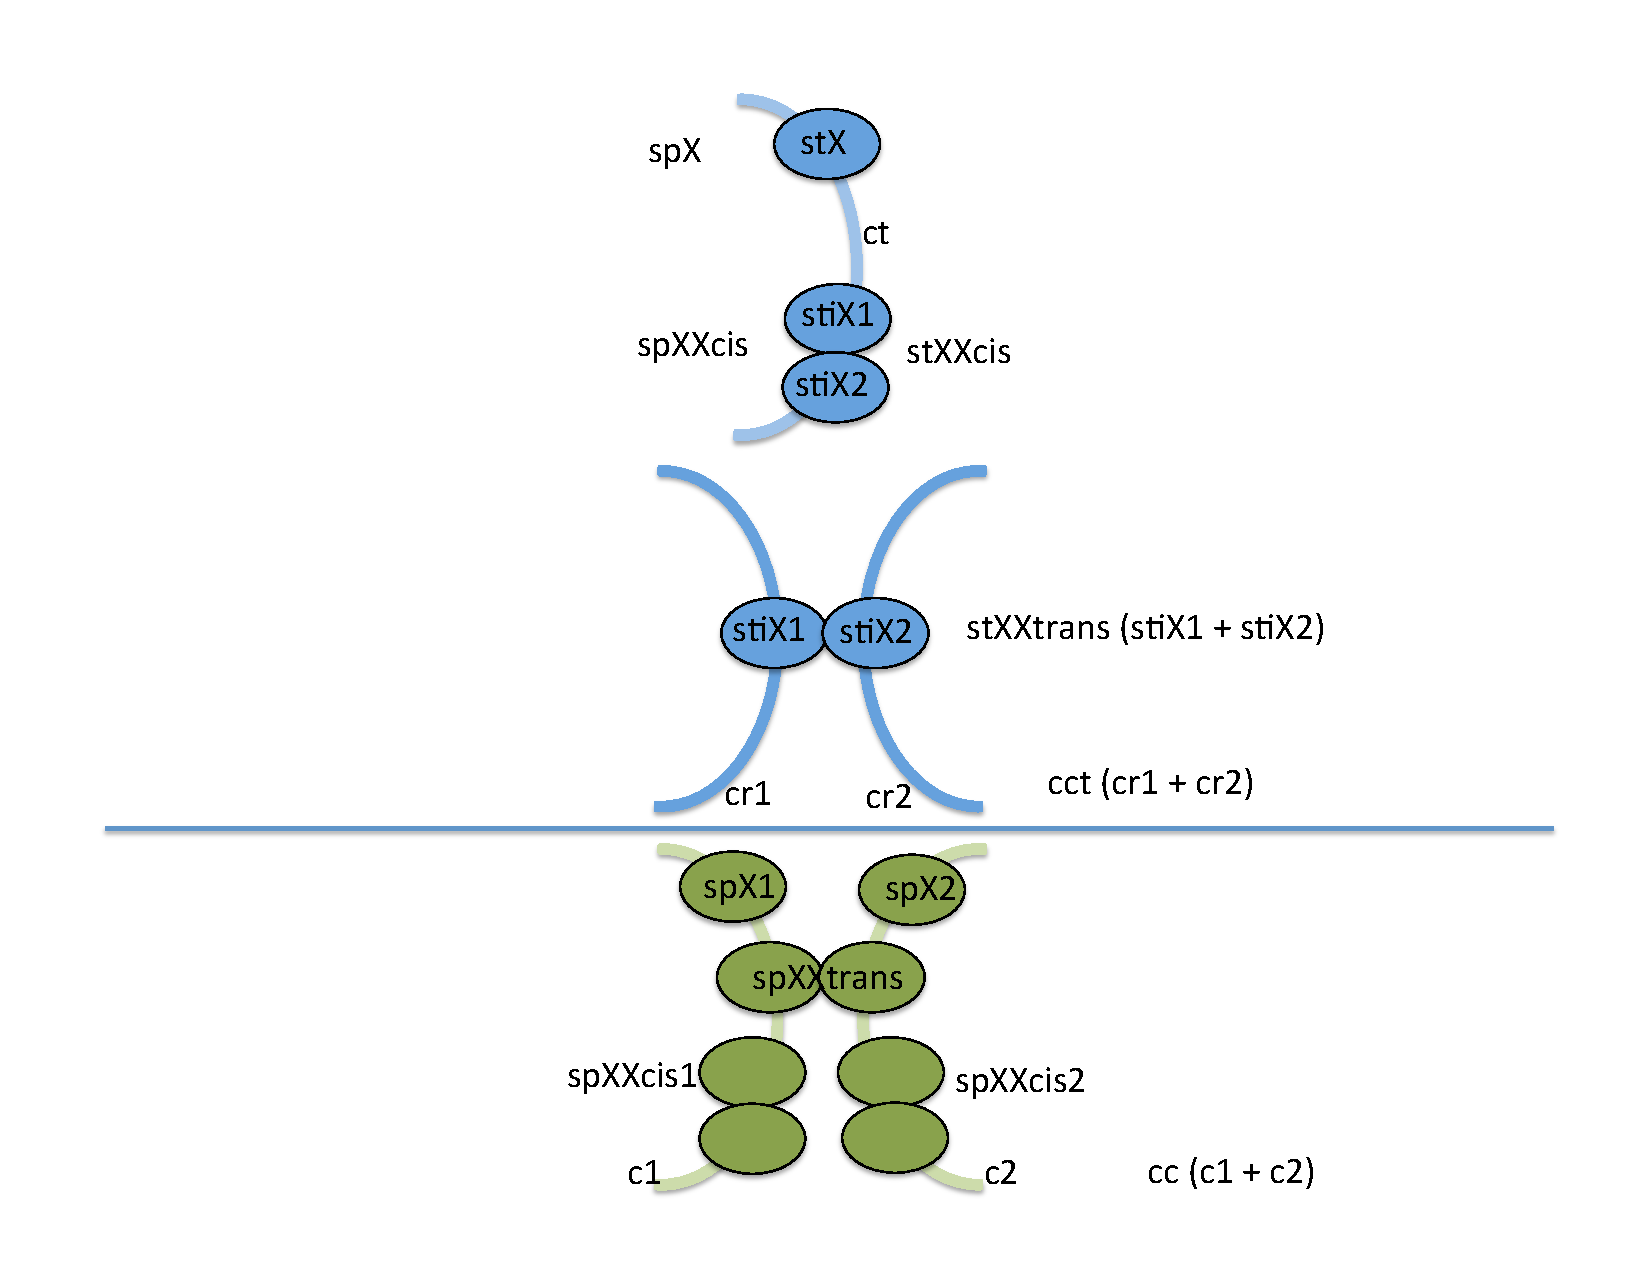
\includegraphics[scale=0.5]{./figs/example_ppt}
  \caption{Diagram for an example of \ExCompartment, \SpeciesType and 
    \ExSpecies}
  \label{fig:Example:CompartmentSpeciesTypeSpecies}
\end{figure}

\fig{fig:Example:CompartmentSpeciesTypeSpecies} shows an example illustrating the usages of and relations among the \ExCompartment, \SpeciesType and \ExSpecies classes. 

\val{ct} is a \compartment\ type. \val{cct} is a composite \compartment\ type with two \compartmentReferences\ \val{cr1} and \val{cr2} both referencing \val{ct}. \val{c1} is a \notatypecompartment\ and references \val{ct}. Similarly, \val{c2} is also a \notatypecompartment\ and references \val{ct}. \val{cc} is a composite \notatypecompartment\ composed of \val{c1} and \val{c2}.

\val{stX} is a \speciesType\ on the \val{ct} \compartment. \val{stXXcis} is a \speciesType\ on the \val{ct} \compartment, and has two \speciesTypeInstances\ \val{stiX1} and \val{stX2} both of that reference the \val{stX} speciesType. \val{stXXtrans} is a \speciesType\ on the \val{cct} \compartment\ with two \speciesTypeInstances\ \val{stiX1} and \val{stiX2} sitting in different sub-compartments.

\val{spX} is a \species\ referencing \speciesType\ \val{stX}. \val{spXXcis} is a \species\ referencing \val{stXXcis}. \val{spX1} is a \species\ referencing \val{stX} and sitting in the \val{c1} \compartment. \val{spX2} is a \species\ also referencing \val{stX}, but sitting in \val{c2}. \val{spXXtrans} is a \species\ referencing \val{stXXtrans}. \val{spXXcis1} is a \species\ referencing \val{stXXtrans} and sitting in \val{c1}.\val{spXXcis1} is a \species\ referencing \val{stXXtrans} and sitting in \val{c2}.

\val{spX1}, \val{spX2}, \val{spXXtrans}, \val{spXXcis1} and \val{spXXcis2} are \fullydefinedspeciesWC.

The SBML code can be as follows:

\exampleFile{./examples/code_002_CompartmentSpeciesTypeSpecies.xml}


%---------------------------------------------
\subsection{\Simmune\ example: the Ecad model} 
\label{def:Example:Simmune:EcadModel}

The \Simmune\  toolset (\url{http://go.usa.gov/QeH}) has some example models including the published \token{Ecad} \model\ [\cite{ref:simmune2012}]. The \token{Ecad} model describes the interactions between \token{E-cadherin} receptors that can associate either with other \token{E-cadherin} receptors within the same membrane (in \val{cis}) or with \token{E-cadherin} receptors on adjacent membranes (in \val{trans}). This model is transformed into the \SbmlLevelThree\ format with use of the \multi\ package.

\exampleFile{./examples/simmune_Ecad.xml}


%------------------------------------------------
\subsection{A \BioNetGen\ example from its user manual}
\label{Example:BioNetGen}

egfr\_simple.bngl (\url{http://bionetgen.org/index.php/BNGManual:Listing_1}) 
% file: bionetgen_egfr_simple.bngl

\begin{example}[style=latex]
begin parameters
  NA 6.02e23                # Avogadro's number (molecules/mol)
  f  1                      # Fraction of the cell to simulate
  Vo f*1.0e-10              # Extracellular volume=1/cell_density (L)
  V  f*3.0e-12              # Cytoplasmic volume (L)
  
  EGF_init 20*1e-9*NA*Vo    # Initial amount of ligand (20 nM)
                            # converted to copies per cell
                            
  # Initial amounts of cellular components (copies per cell)
  EGFR_init f*1.8e5
  Grb2_init f*1.5e5
  Sos1_init f*6.2e4

  # Rate constants
  # Divide by NA*V to convert bimolecular rate constants
  # from /M/sec to /(molecule/cell)/sec
  kp1 9.0e7/(NA*Vo)   # ligand-monomer binding
  km1 0.06            # ligand-monomer dissociation
  kp2 1.0e7/(NA*V)    # aggregation of bound monomers
  km2 0.1             # dissociation of bound monomers
  kp3 0.5             # dimer transphosphorylation
  km3 4.505           # dimer dephosphorylation
  kp4 1.5e6/(NA*V)    # binding of Grb2 to receptor
  km4 0.05            # dissociation of Grb2 from receptor
  kp5 1.0e7/(NA*V)    # binding of Grb2 to Sos1
  km5 0.06            # dissociation of Grb2 from Sos1
  deg 0.01            # degradation of receptor dimers
end parameters

begin molecule types
  EGF(R)
  EGFR(L,CR1,Y1068~U~P)
  Grb2(SH2,SH3)
  Sos1(PxxP)
  Trash()
end molecule types

begin seed species
  EGF(R)              0
  EGFR(L,CR1,Y1068~U) EGFR_init
  Grb2(SH2,SH3)       Grb2_init
  Sos1(PxxP)          Sos1_init
end seed species

begin observables
  1 Molecules   EGFR_tot  EGFR()
  2 Molecules   Lig_free  EGF(R)
  3 Species     Dim       EGFR(CR1!+)
  4 Molecules   RP        EGFR(Y1068~P!?)
  5 Molecules   Grb2Sos1  Grb2(SH2,SH3!1).Sos1(PxxP!1)
  6 Molecules   Sos1_act  EGFR(Y1068!1).Grb2(SH2!1,SH3!2).Sos1(PxxP!2)
end observables

begin reaction rules
  # Ligand-receptor binding
  1 EGFR(L,CR1) + EGF(R) <-> EGFR(L!1,CR1).EGF(R!1) kp1, km1
  
  # Receptor-aggregation
  2 EGFR(L!+,CR1) + EGFR(L!+,CR1) <-> EGFR(L!+,CR1!1).EGFR(L!+,CR1!1) kp2,km2
  
  # Transphosphorylation of EGFR by RTK
  3 EGFR(CR1!+,Y1068~U) -> EGFR(CR1!+,Y1068~P) kp3
  
  # Dephosphorylation
  4 EGFR(Y1068~P) -> EGFR(Y1068~U) km3
  
  # Grb2 binding to pY1068
  5 EGFR(Y1068~P) + Grb2(SH2) <-> EGFR(Y1068~P!1).Grb2(SH2!1) kp4,km4
  
  # Grb2 binding to Sos1
  6 Grb2(SH3) + Sos1(PxxP) <-> Grb2(SH3!1).Sos1(PxxP!1) kp5,km5
  
  # Receptor dimer internalization/degradation
  7 EGF(R!1).EGF(R!2).EGFR(L!1,CR1!3).EGFR(L!2,CR1!3) -> Trash()
end reaction rules

#actions
generate_network({overwrite=>1});

# Equilibration
simulate_ode({suffix=>equil,t_end=>100000,n_steps=>10,sparse=>1,steady_state=>1});
setConcentration("EGF(R)","EGF_init");
saveConcentrations(); # Saves concentrations for future reset

# Kinetics
writeSBML({});
simulate_ode({t_end=>120,n_steps=>120});
resetConcentrations(); # reverts to saved Concentrations
simulate_ssa({suffix=>ssa,t_end=>120,n_steps=>120});
\end{example}

The SBML code can be as follows. Please note, the SBML code does not cover the content other than the model in the bngl file, such as the \val{actions}, \val{Equilibration} and \val{Kinetics} sections.

\exampleFile{./examples/bionetgen_egfr_simple.xml}

%------------------------------------------------
\subsection{Example from \Kappa 's documentation}
\label{def:Example:Kappa}

Here is the example ``An Introduction to Kappa Syntax'' at \Kappa\ website 
(\url{http://www.kappalanguage.org/syntax.html}).

Rule in English: ``Unphosphorylated Site1 of A binds to Site1 of B''

Kappa Rule: \objFont{A(Site1~u),B(Site1) -> A(Site1~u!1),B(Site1!1)}

\exampleFile{./examples/kappa_introduction_syntax.xml}

\clearpage